\documentclass[times, utf8, zavrsni]{fer}
\usepackage{booktabs}
\usepackage{pdfpages}
\usepackage{listings}

\renewcommand{\lstlistingname}{Isječak}

\begin{document}

\lstset{
basicstyle=\ttfamily\footnotesize,
keepspaces=true,
numbers=left,
frame=single,
captionpos=b,
showspaces=false,
numberstyle=\ttfamily,
columns=flexible
}

\thesisnumber{5709}

\title{Sustav za određivanje strukture teksta na temelju položaja pojedinih znakova}

\author{Herman Zvonimir Došilović}

\maketitle

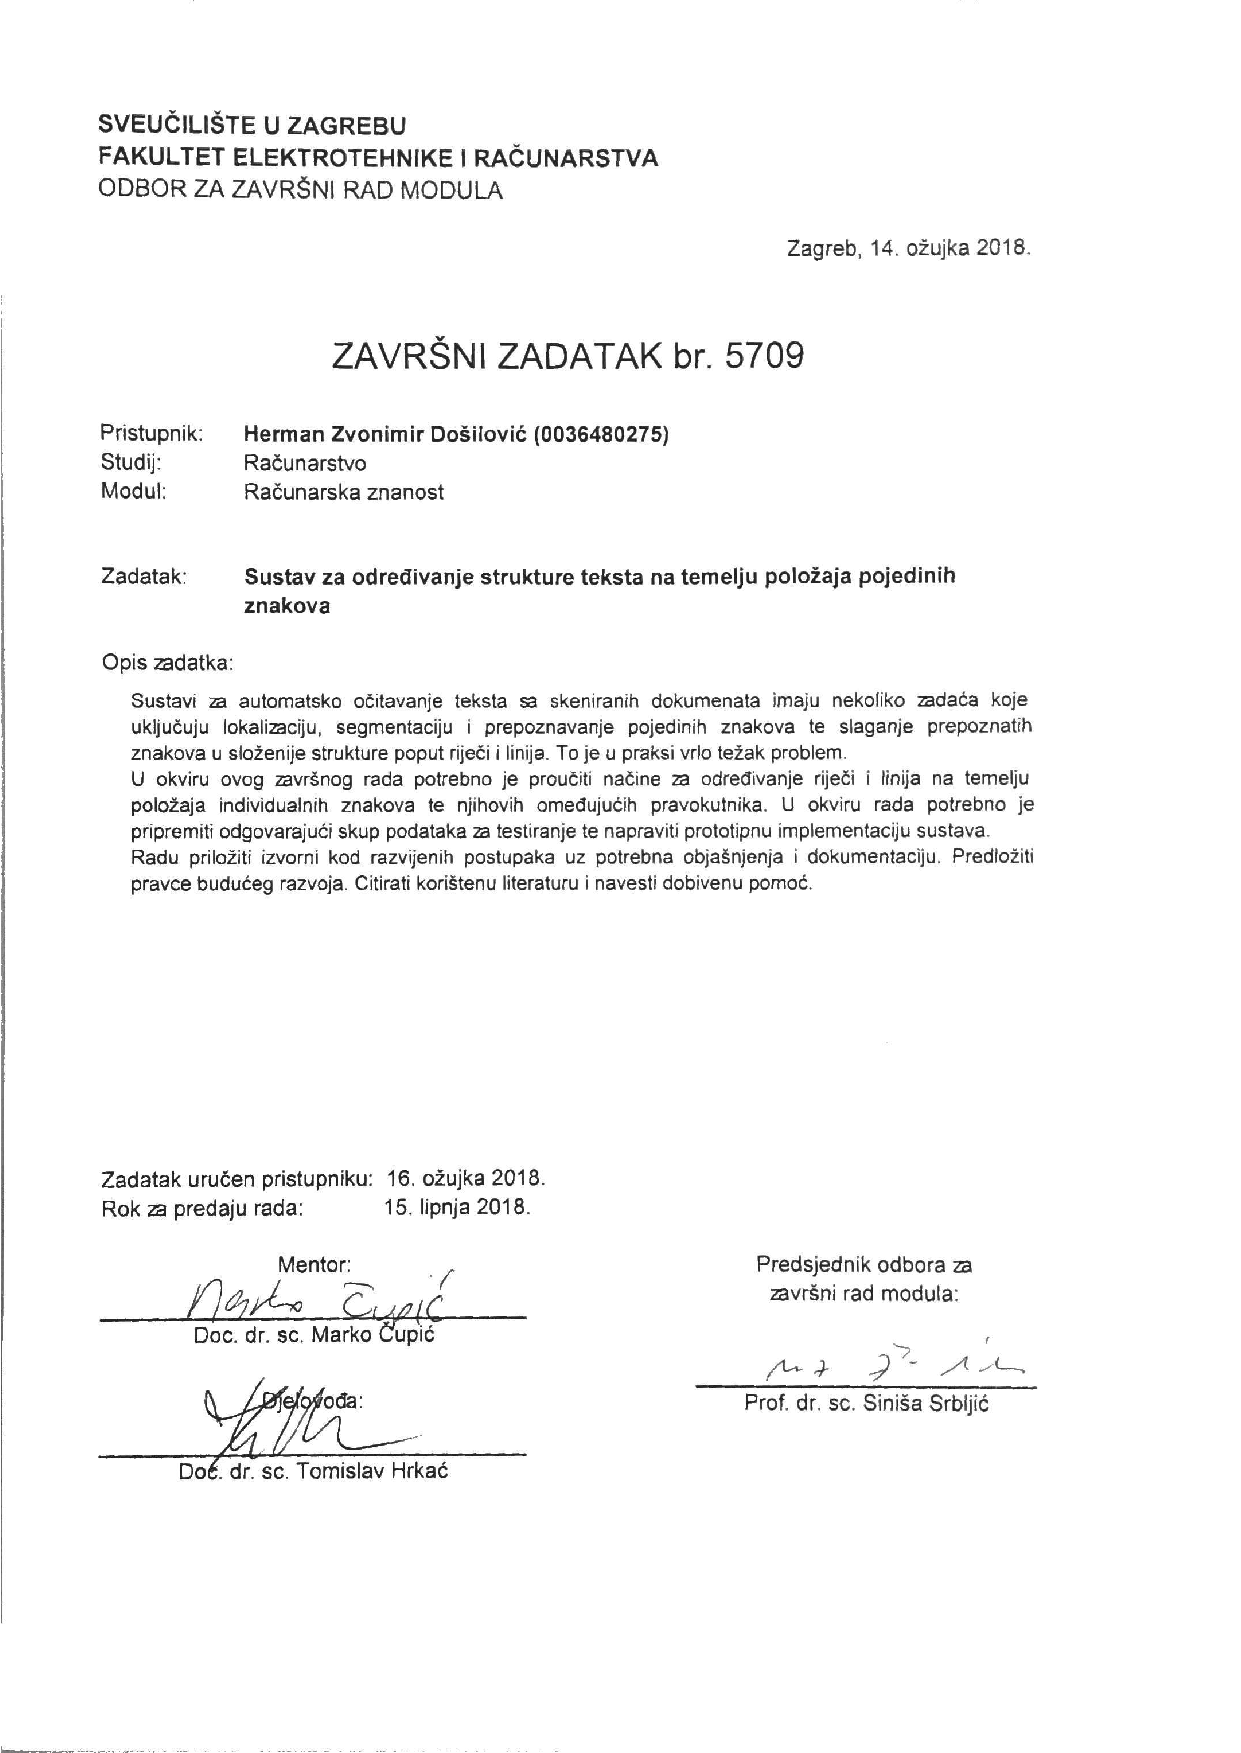
\includepdf[pages=-]{izvornik.pdf}

\zahvala{
    Zahvaljujem svom mentoru doc. dr. sc. Marku Čupiću na dozvoli za odabir vlastite teme i
    na strpljenju, poticaju i savjetima u razvoju rada.

    \

    Zahvaljujem tvrtki Microblink na danim sredstvima bez kojih ovaj rad ne bi bio moguć.
    Posebno zahvaljujem kolegama Jurici Cerovecu, Nenadu Mikši, Borisu Trubiću,
    Igoru Smolkoviču i Ivanu Jurinu koji su me svojim bogatim znanjem i iskustvom
    usmjeravali u razvoju rada.
}

\zahvala{
    Tko hoće da među vama bude najveći, neka vam bude poslužitelj! I tko hoće da
    među vama bude prvi, neka bude svima sluga. - Mk 10,43-44
}

\tableofcontents

\chapter{Uvod}
\chapter{Optičko raspoznavanje znakova}
Sustav za optičko raspoznavanje znakova \engl{optical character recognition} (u daljnjem tekstu: OCR)
pretvara sliku tiskanog teksta u digitalizirani format kojim možemo jednostavno manipulirati na računalu.
Iako je to ljudima jednostavan zadatak, računalima nije lako prepoznati tekst i pojedine znakove teksta sa slike
zbog velike raznolikosti jezika, fonta i stila kojim tekst može biti napisan.
OCR je stoga vrlo zahtjevan problem i mnogo je istraživačkog truda uloženo u pokušaju
da se slike teksta pretvore u format koji računalo razumije. \citep{DBLP:journals/corr/abs-1710-05703}

\section{Primjene}

Osim tiskanog teksta, OCR sustavi koriste se i u prepoznavanju znakova rukom pisanog teksta.
Prepoznavanje znakova rukom pisanog teksta je teži problem od prepoznavanja tiskanog teksta \citep{DBLP:journals/corr/abs-1710-05703} zato jer
se oblik znakova i njihov način pisanja razlikuje kod svake osobe (npr. rukopis odrasle osobe potpuno je drugačiji od
rukopisa djeteta).
OCR sustave za detekciju rukom pisanih znakova možemo podijeliti na dvije potkategorije:
\emph{on-line} i \emph{off-line}. \emph{On-line} OCR sustavi detektiraju znakove dok
ih korisnici unose i to im omogućuje praćenje parametara poput: brzine pisanja, broj napravljenih poteza,
smjer pisanja, itd. \emph{Off-line} OCR sustavi izvode se nad jednom slikom na kojoj se nalazi
sav sadržaj nad kojim je potrebno napraviti detekciju. Takvi sustavi nemaju dodatne informacije koje imaju
\emph{on-line} sustavi i zato je detekcija znakova kompliciranija \citep{DBLP:journals/corr/abs-1710-05703}. Slika \ref{fig:math-example-01} prikazuje primjer rezultata
\emph{off-line} OCR sustava za detekciju rukom pisanih znakova.

\begin{figure}[htb]
    \centering
    \captionsetup{justification=centering,margin=2cm}
    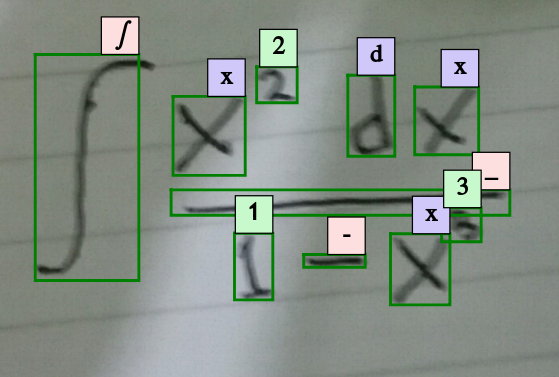
\includegraphics[height=4cm]{images/math-example-01.png}
    \caption{Rezultat \emph{off-line} OCR sustava za detekciju znakova rukom pisanog teksta.}
    \label{fig:math-example-01}
\end{figure}

\pagebreak

OCR sustavi imaju široku primjenu i možemo ih pronaći primjerice u detekciji
znakova na registarskim pločicama \citep{DBLP:journals/corr/Saghaei16a}, \citep{DBLP:journals/corr/abs-1802-09567},
u detekciji znakova na tiskanim knjigama \citep{DBLP:journals/corr/abs-1802-10033},
\citep{Christy:2017:MDE:3172938.3075645} i
detekciji znakova na raznim dokumenatima \citep{DBLP:journals/corr/HarrajR15} \citep{verma2016ocr}. Na slici \ref{fig:receipt-example-01}
prikazan je primjer rezultata korištenja OCR sustava za detekciju znakova na računima iz trgovine.
Slika \ref{fig:book-example-01} prikazuje rezultat OCR sustava za detekciju znakova na tiskanim knjigama.

\begin{figure}[htb]
    \centering
    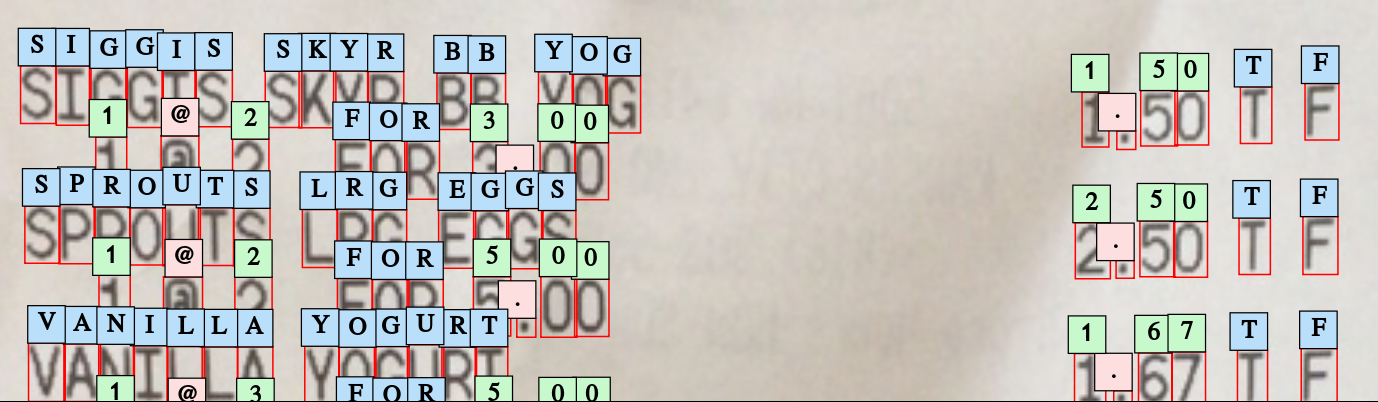
\includegraphics[width=\textwidth]{images/receipt-example-01.png}
    \caption{Rezultat OCR sustava za detekciju znakova na računima iz trgovine.}
    \label{fig:receipt-example-01}
\end{figure}

\begin{figure}[htb]
    \centering
    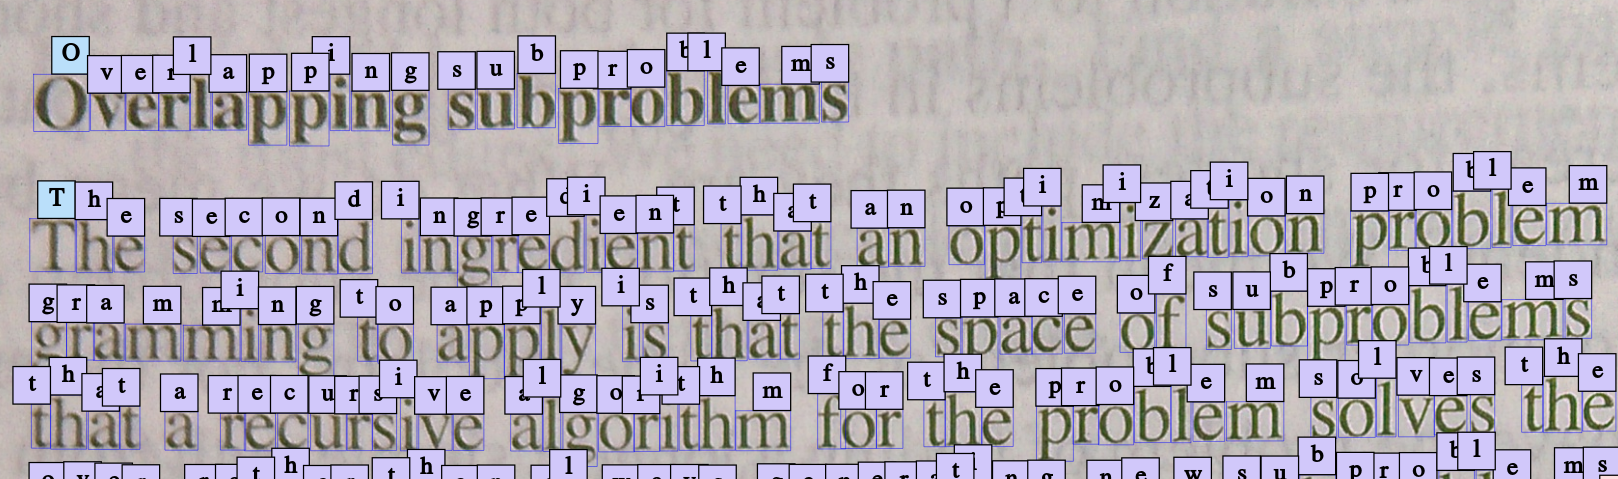
\includegraphics[width=\textwidth]{images/book-example-01.png}
    \caption{Rezultat OCR sustava za detekciju znakova na tiskanim knjigama.}
    \label{fig:book-example-01}
\end{figure}

\pagebreak

\section{Proces izvođenja}

Optičko raspoznavanje znakova provodi se u nekoliko koraka \citep{DBLP:journals/corr/abs-1710-05703} \citep{kaur2016survey}:
\begin{enumerate}
    \item pribavljanje slike,
    \item pretprocesiranje,
    \item segmentacija znakova,
    \item izdvajanje značajki znakova,
    \item klasifikacija znakova i
    \item postprocesiranje.
\end{enumerate}

\subsubsection{Pribavljanje slike}

U prvom koraku OCR-a, pribavljanju slike, potrebno je pribaviti sliku nad kojom ćemo
provesti ostale korake. Sliku možemo pribaviti s raznih uređaja poput kamere fotoaparata,
mobilnog uređaja ili nekog drugog uređaja za digitalizaciju dokumenata \engl{scanner}.
Nakon prvog koraka, slika dokumenta nad kojim provodimo raspoznavanje znakova sastoji se
samo od slikovnih elemenata \engl{pixels} \citep{Vynckier:2018:HowOcrWorks}.
Slika \ref{fig:receipt-example-02} prikazuje primjer slike nad kojom možemo provesti
postupak raspoznavanja znakova. Primjetimo da slika može sadržati pozadinu koju bi
OCR sustav trebao zanemariti.

\begin{figure}[htb]
    \centering
    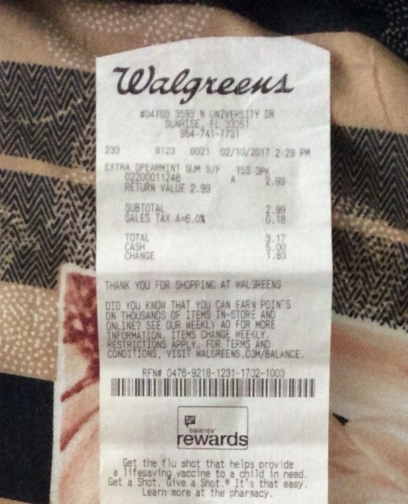
\includegraphics[height=7cm]{images/receipt-example-02.jpeg}
    \caption{Ulazna slika u OCR sustav pribavljena kamerom mobilnog uređaja.}
    \label{fig:receipt-example-02}
\end{figure}

\subsubsection{Pretprocesiranje}

U koraku pretprocesiranja slike OCR sustavi često provode niz morfoloških transformacija i filtra nad pribavljenom slikom.
Cilj ovog koraka je povećati kvalitetu slike i smanjiti informacije na slici. Binarizacija je jedan od
potkoraka pretporocesiranja koji slike u boji ili u nijansama sive pretvara u crno-bijele. Osim binarizacije
koriste se neke morfološke transformacije poput dilatacije, rezanja i skaliranja.
Slika \ref{fig:binarization} prikazuje primjer slike prije i nakon binarizacije. \citep{Gulan:2016:Bacherlor},
\citep{DBLP:journals/corr/abs-1710-05703}, \citep{Jurin:2017:Master}

\begin{figure}[htb]
    \centering
    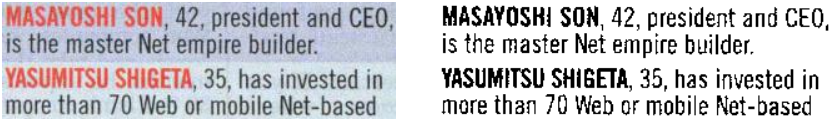
\includegraphics[width=\textwidth]{images/binarization.png}
    \caption{Prije binarizacije (lijevo) i nakon binarizacije (desno) \citep{Vynckier:2018:HowOcrWorks}.}
    \label{fig:binarization}
\end{figure}

\subsubsection{Segmentacija znakova}
\label{subsubsec:segmentacija}

Sljedeći korak, segmentacija znakova, je postupak segmentiranja slike u segmente unutar kojih se nalaze znakovi
koje želimo klasificirati. Jedan od pristupa segmentacije izvodi se s vrha prema dnu gdje se najprije
segmentiraju linije, zatim riječi i na kraju pojedini znakovi \citep{Jurin:2017:Master}, \citep{Vynckier:2018:HowOcrWorks}.
Prednost ovakvog pristupa je da uz lokaciju svakog znaka dobivamo i strukturu cijelog teksta, odnosno, znamo kojoj
liniji i kojoj riječi znak pripada. Nedostatak ovakvog pristupa je da ne postoje korekcijski mehanizmi kojima bismo
znak pridružili nekoj drugoj liniji ili riječi ako su prva dva koraka segmentacije linije ili riječi neispravni. \citep{Jurin:2017:Master}

Drugi pristupi poput \emph{ZICER OCR}\footnote{OCR sustav tvrtke \emph{Microblink}, \url{https://microblink.com}} sustava izravno
izvode segmentaciju cijele slike na području koji predstavljaju znakove. Prednost takvog pristupa je da
možemo detektirati znakove teksta u kojemu nema riječi i linija, kao što je na primjer matematički izraz.
Nedostatak takvog pristupa je da gubimo informaciju o strukturi teksta i zato postoji potreba za razvojem dodatnog sustava koji bi znakove
grupirao u riječi, a riječi u linije \citep{Jurin:2017:Master}.
Slika \ref{fig:segmentation} prikazuje rezultat segmentacije pojedinih znakova.

\begin{figure}[htb]
    \centering
    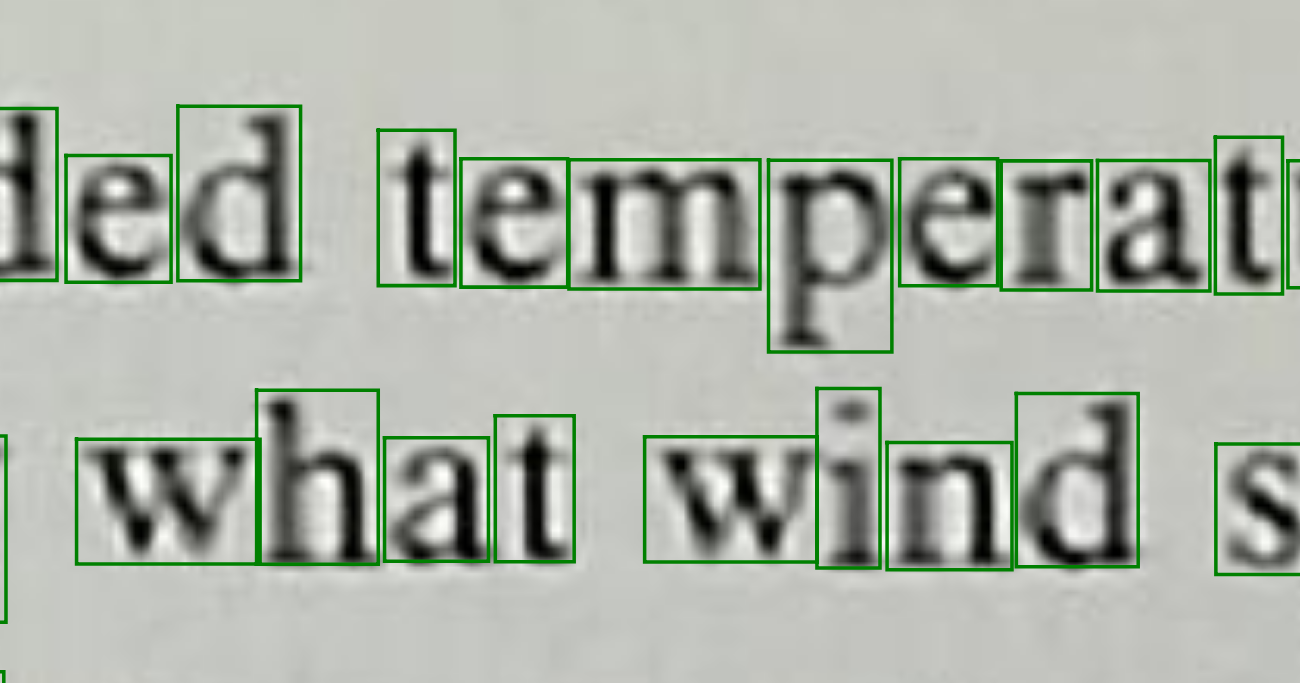
\includegraphics[height=4cm]{images/segmentation.png}
    \caption{Segmentacija znakova.}
    \label{fig:segmentation}
\end{figure}

\pagebreak

\subsubsection{Izdvajanje značajki}

Izdvajanje značajki pojedinog znaka podrazumijeva odabir značajki prema kojima će
se jedinstveno klasificirati svaki znak. Značajke poput geometrijskog oblika ili
statističkih svojstava mogu biti uzete u obzir prilikom klasifikacije. Važno područje istraživanja pripada
razmatranju koje i koliko značajki je potrebno uzeti u obzir za kvalitetnu i ispravnu
klasifikaciju. \citep{DBLP:journals/corr/abs-1710-05703}

\subsubsection{Klasifikacija}

Klasifikacija je najvažniji korak optičkog raspoznavanja znakova \citep{verma2012survey} \citep{zhu2016novel}
koji koristi izdvojene značajke za određivanje klase pojedinog znaka \citep{lehal1999feature} \citep{kaur2016survey}.
Statistički pristupi klasifikacije koriste diskriminativne funkcije za određivanje klase znaka \citep{DBLP:journals/corr/abs-1710-05703},
a u novije vrijeme koriste se duboke neuronske mreže \citep{Jurin:2017:Master}.
Neki od statističkih pristupa su: Bayesov klasifikator, klasifikator stablom odluke, umjetne neuronske mreže i
metoda k-najbližih susjeda \citep{DBLP:journals/corr/abs-1710-05703}.

2012. godine Krizhevsky i suradnici \citep{krizhevsky2012imagenet} objavili su rad koji je
označio prekretnicu u klasifikaciji i lokalizaciji objekata \citep{Jurin:2017:Master}. Slika
\ref{fig:deep-example-01} prikazuje arhitekturu \emph{AlexNet} koja je pobijedila na natječaju
\emph{ImageNet 2012} u području klasifikacije objekata. \citep{Jurin:2017:Master}

\begin{figure}[htb]
    \centering
    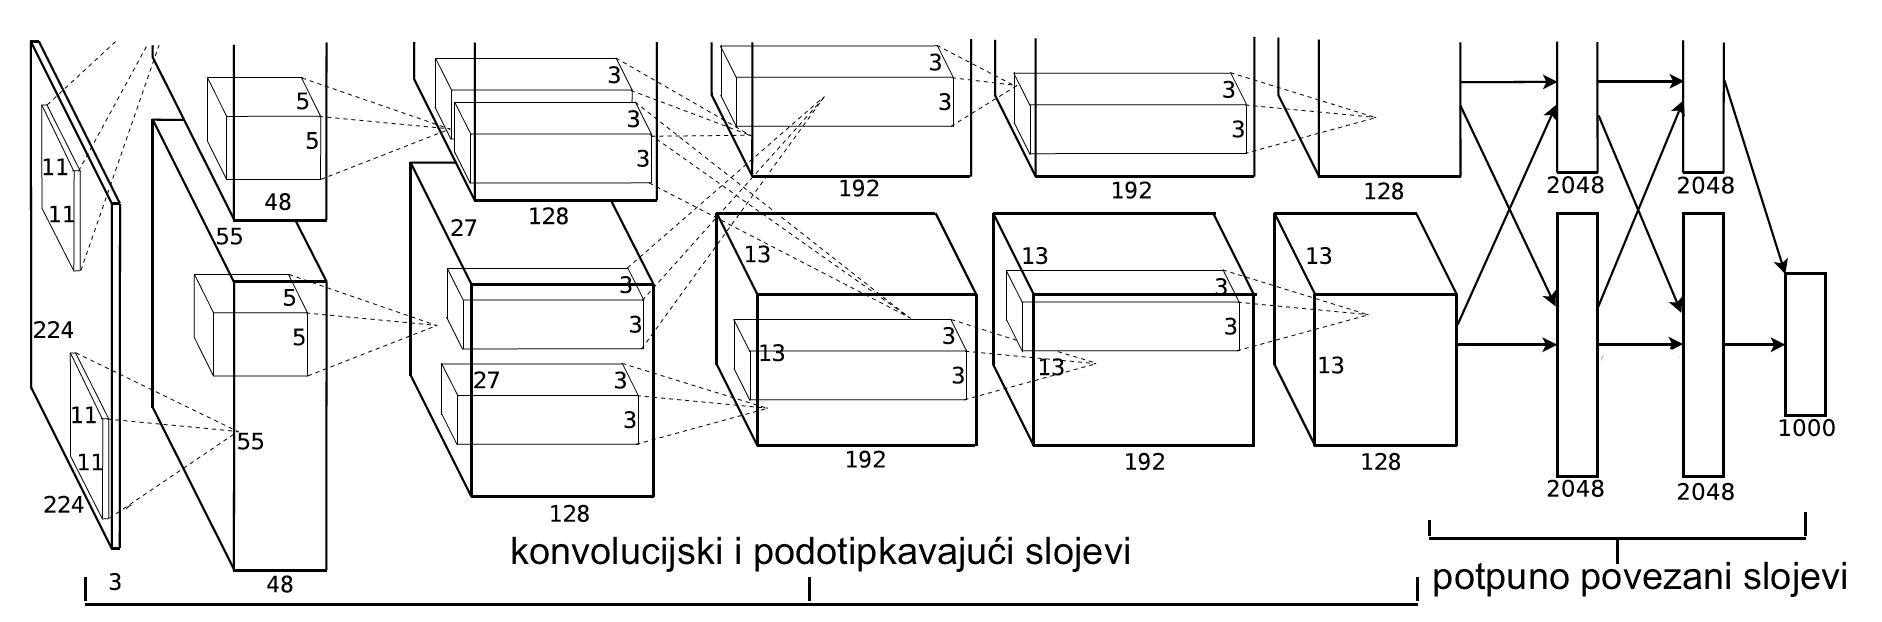
\includegraphics[width=\textwidth]{images/deep-example-01.png}
    \caption{Arhitektura \emph{AlexNet} \citep{Jurin:2017:Master}}
    \label{fig:deep-example-01}
\end{figure}

\subsubsection{Postprocesiranje}

Nakon klasifikacije znakova slijedi njihovo postprocesiranje koje se koristi kako
bi se poboljšali rezultati OCR-a. Jedan od pristupa postprocesiranja koristi rezultate
više različitih klasifikatora koji mogu biti korišteni slijedno, paralelno ili hijerarhijski.
Nakon toga rezultati klasifikatora se kombiniraju različitim pristupima. \citep{DBLP:journals/corr/abs-1710-05703}
Kao što je spomenuto u \ref{subsubsec:segmentacija} segmentacija koja se ne provodi s vrha prema
dnu nema informaciju o strukturi teksta i zato je potrebno razviti dodatan
\textbf{sustav za određivanje strukture teksta na temelju položaja pojedinih znakova}.

Schulz i suradnici \citep{schulz2017multi} 2017. godine predstavili su arhitekturu
tzv. \emph{post-correction} OCR sustava kojim su pokazati na koji način su
adaptirali generički sustav za postprocesiranje OCR rezultata koristeći domensko znanje
za konkretan problem koji su rješavali. Ovim pristupom ostvarili su bolje rezultate
za konkretni problem nego što su ostvarili koristeći postojeći generički sustav za
postprocesiranje OCR rezultata.

\

\begin{figure}[htb]
    \centering
    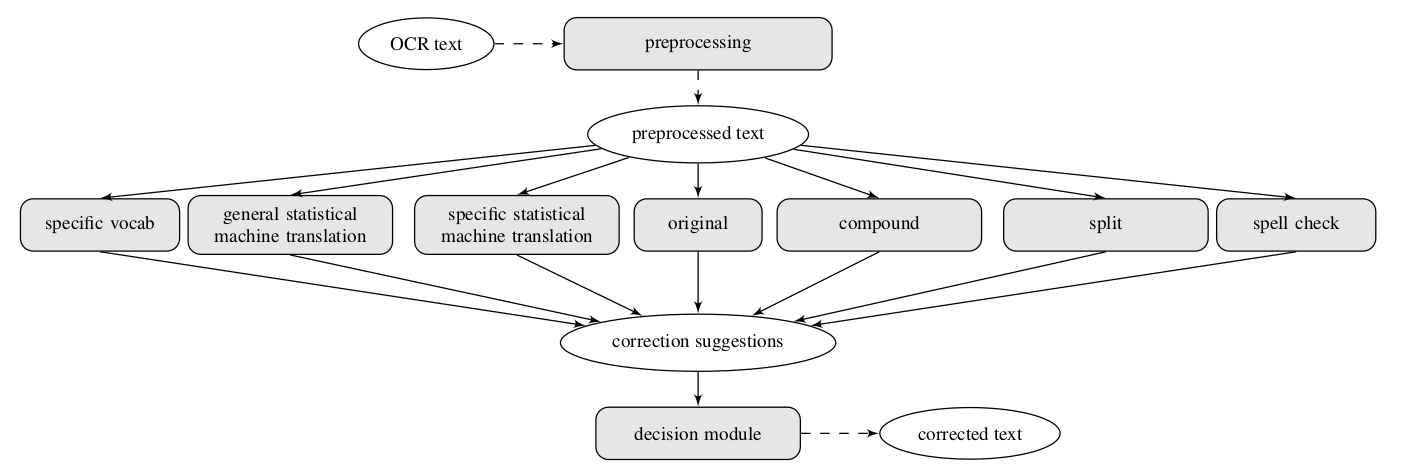
\includegraphics[width=\textwidth]{images/post-correction-example-01.png}
    \caption{Arhitektura \emph{post-correction} OCR sustava \citep{schulz2017multi}}
    \label{fig:post-correction-example-01}
\end{figure}

\chapter{Određivanje strukture teksta}
Sustavi za određivanje strukture teksta na temelju OCR rezultata sastavni su dio OCR sustava. Određivanje strukture teksta
podrazumjeva segmentaciju linija i segmentaciju riječi unutar linije. Neke tehnike segmentacije
OCR znakova i njihove klasifikacije nemaju informaciju o tome kojoj liniji i riječi pojedini znak pripada.
Prednost takvog pristupa je da takav OCR sustav možemo koristiti nad slikama koje ne sadrže linije,
kao na primjer matematički izrazi \citep{Jurin:2017:Master}. Nedostatak je što nakon klasifikacije
moramo razviti sustav koji će OCR znakove dodatno procesirati da bismo dobili strukturu teksta \citep{Jurin:2017:Master}.

Tekst na slici može biti podijeljen na linije ili blokove, a u bloku
tekst možemo podijeliti na linije. Unutar jedne linije znakove možemo grupirati riječi. Način na
koji će se odrediti struktura teksta uvelike ovisi o problemu koji riješavamo i kakve rezultate
želimo dobiti.

Tain i suradnici \citep{DBLP:journals/corr/TianPHLYT16} predlažu sustav za određivanje strukture teksta
koji će osim određivanja kojoj liniji pojedini znak pripada znati izbaciti tzv. \emph{false positive}
znakove odnosno znakove koje je OCR sustav prepoznao, a zapravo u tekstu ne postoje. Njihov sustav temelji
se na \emph{min-cost flow network} modelu koji objedinjuje izbacivanje \emph{false positive} znakova i
pronalazak strukture teksta. Na temelju međusobne pozicije između dva prepoznata znaka i
dodatnog parametra kojeg dobivaju od klasifikatora, a koji označava vjerojatnost ispravne detekcije, grade težinski
usmjereni graf (Slika \ref{fig:text-flow}) koji svoj problem modeliraju \emph{min-cost flow network} modelom.

\begin{figure}[htb]
    \centering
    \captionsetup{justification=centering,margin=2cm}
    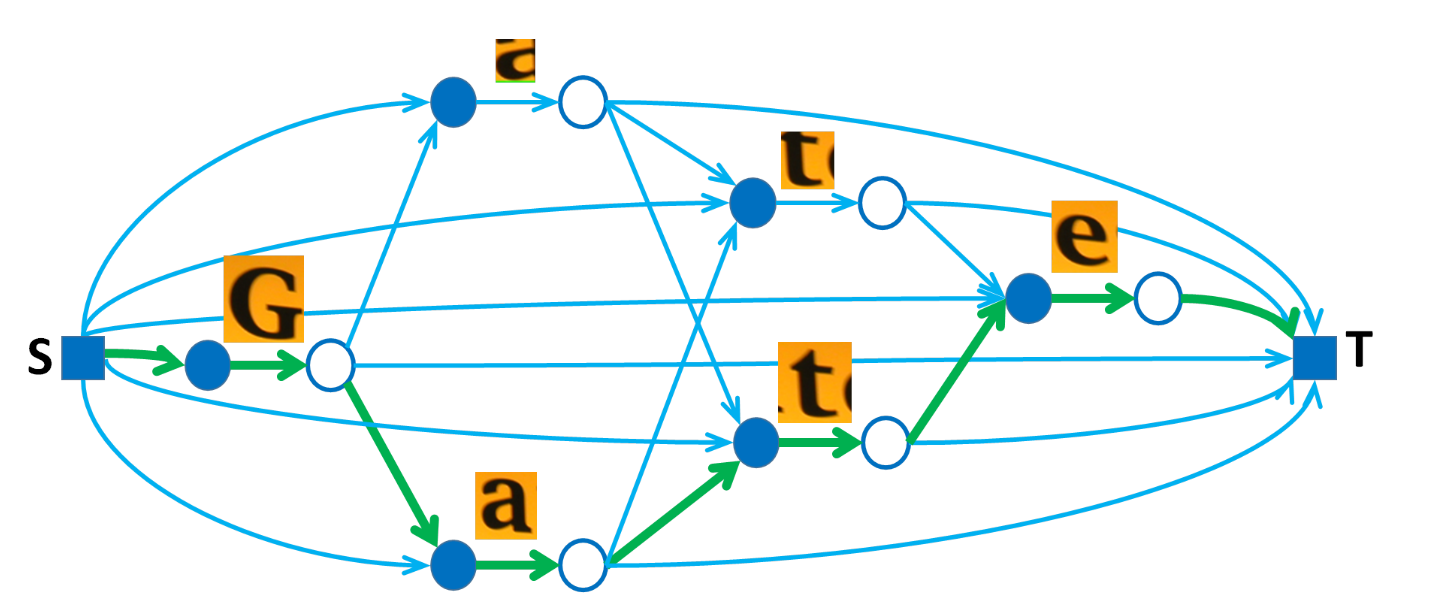
\includegraphics[height=6cm]{images/text-flow.png}
    \caption{Težinski usmjereni graf temeljen na \emph{min-cost flow network} modelu \citep{DBLP:journals/corr/TianPHLYT16}.}
    \label{fig:text-flow}
\end{figure}

\pagebreak

Zhu i suradnici \citep{zhu2016novel} predložili su novu arhitekturu (Slika \ref{fig:novel-ocr}) OCR sustava koji se temelji na empirijskim
rezultatima koji su pokazali da sadržaj riječi ne ovisi samo o dijelu teksta u kojem se ta riječ
nalazi nego i o susjednim dijelovima teksta. Njihov novi OCR sustav radi dvostruku analizu strukture
teksta -- prije klasifikacije i nakon klasifikacije. Prva analiza strukture teksta omogućuje im da odrede
strukturu teksta u blokovima, a druga analiza strukture teksta im omogućuje da poprave pogreške u klasifikaciji.
Njihova nova arhitektura predstavlja hibridni OCR sustav koji iskorištava rezultate analize strukture teksta.

\

\begin{figure}[htb]
    \centering
    \captionsetup{justification=centering,margin=2cm}
    \fbox{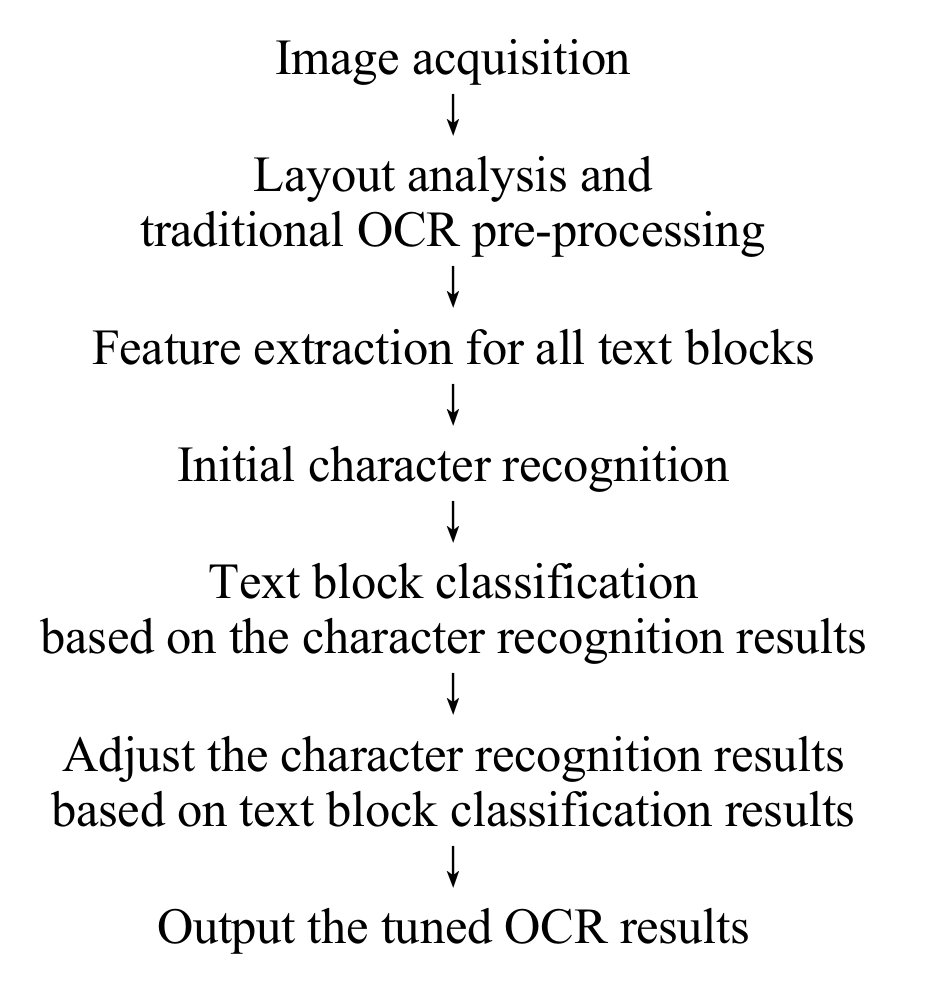
\includegraphics[height=7cm]{images/novel-ocr.png}}
    \caption{Arhitektura novog OCR sustava kojeg predlažu Zhu i suradnici \citep{zhu2016novel}.}
    \label{fig:novel-ocr}
\end{figure}

\pagebreak

Yin i suradnici \citep{yin2007handwritten} pronalaze linije u tekstu povezujući znakove u težinski
graf nad kojim provode Kruskalov algoritam za pronalazak minimalnog razapinjujućeg stabla. Njihov
pristup ne koristi rezultate klasifikacije, nego koriste povezane komponente koje im predstavljaju
znakove i koje pronalaze koristeći algoritam temeljen na praćenju kontura \engl{contour tracing}.
Slika \ref{fig:mst-example-01} prikazuje rezultat pronalaska linija teksta u rukom pisanom dokumentu na
Engleskom jeziku.

\

\begin{figure}[htb]
    \centering
    \captionsetup{justification=centering,margin=2cm}
    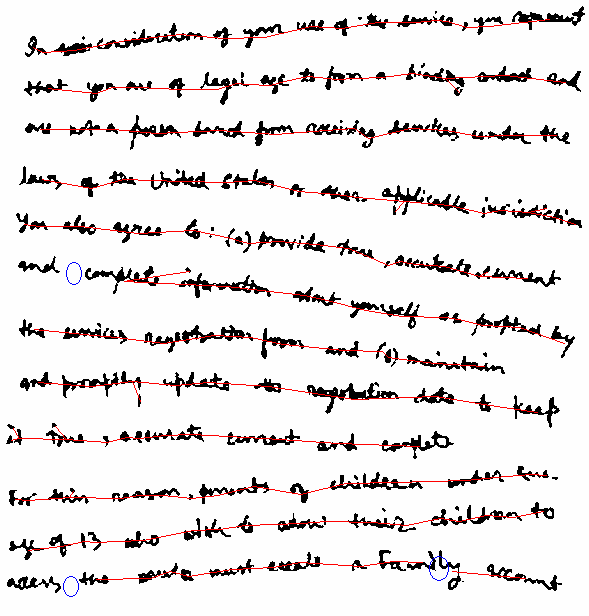
\includegraphics[height=8cm]{images/mst-example-01.png}
    \caption{Rezultat pronalaska linija teksta u rukom pisanom dokumentu na Engleskom jeziku \citep{yin2007handwritten}}
    \label{fig:mst-example-01}
\end{figure}

Motivirani njihovim radom Pan i suradnici \citep{pan2011hybrid} predstavili su sličan pristup
koji u težinama grafa uzima u obzir dodatne težine koje su učene MCE \engl{minimum classification error} mjerom.

Još jedan pristup predložili su Yin i suradnici \citep{DBLP:journals/corr/abs-1301-2628} koji koriste
tehniku hijerahijskog grupiranja koji postupno spaja linije koje dijele znakove dok god
postoje linije koje se mogu spojiti. \citep{DBLP:journals/corr/TianPHLYT16}

Liang i suradnici \citep{liang1996document} predlažu heuristički algoritam za određivanje sturkture
teksta. Algoritam radi horizontalnu projekciju (Slika \ref{fig:histogram-projection}) omeđujućih pravokutnika na jednu ravninu i pronalazi
vrhove i doline u histogramu koji prikazuje frekvencije pojavljivanja projektiranih pravokutnika.
Osim ovog pristupa predložili su još jedan koji spaja dva znaka u jednu cjelinu ako i samo ako
su dva znaka dovoljno blizu da ih ima smisla spojiti. Gupta i suradnici \citep{gupta2006document} također koriste razne heuristike prema kojima
povezuju susjedne omeđujuće pravokutnike.

\pagebreak

\begin{figure}[htb]
    \centering
    \captionsetup{justification=centering,margin=2cm}
    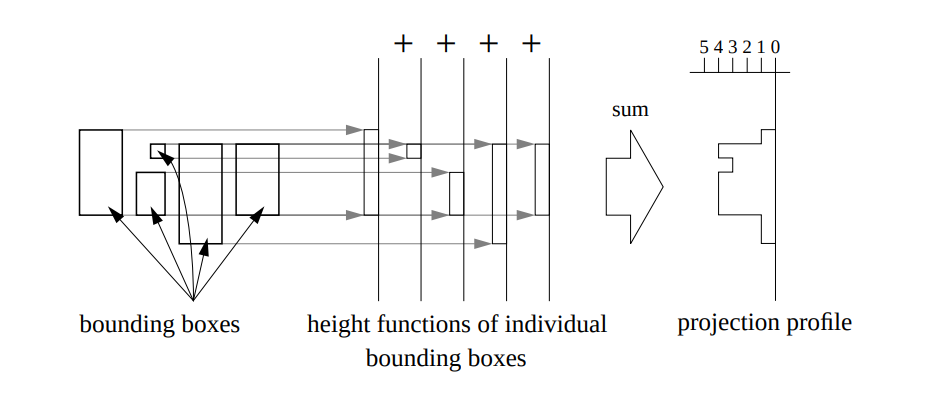
\includegraphics[height=6cm]{images/histogram-projection.png}
    \caption{Histogram dobiven horizontalnom projekcijom omeđujućih pravokutnika \citep{liang1996document}}
    \label{fig:histogram-projection}
\end{figure}

Određivanje strukture teksta težak je postupak koji uvelike ovisi o problemu koji rješavamo. U ovom
poglavlju smo pokazali da strukturiranje teksta može biti izvođeno u raznim fazama izvođenja OCR
sustava. Trenutak u kojem ćemo pokrenuti analizu strukture teksta ovisi o načinu na koji smo
označili segmente znakova, koje informacije o segmentu imamo i koji problem rješavamo.
Pokazali smo da su neki pristupi postigli bolje rezultate kada se iskoristilo domensko znanje
i kada su se u nekim heurističkim pristupima koristili parametri koji su bili pomno
izabrani za dani problem.
U nastavku ovog rada predložiti ćemo nekoliko pristupa za određivanje strukture teksta na temelju položaja omeđujućih pravokutnika nakon provedene klasifikacije
znakova. Analizirati ćemo njihove prednosti i nedostatke i cijelo vrijeme ćemo znati koji točno problem rješavamo.

\chapter{Opis problema}
Problem koji rješavamo je određivanje strukture teksta na temelju položaja pojedinih znakova.
Od OCR sustava dobijemo listu znakova i za svaki znak znamo sljedeće informacije:
\begin{itemize}
    \item[$\bullet$] $x$ - horizontalnu poziciju gornjeg lijevog kuta,
    \item[$\bullet$] $y$ - vertikalnu poziciju gornjeg lijevog kuta,
    \item[$\bullet$] $width$ - širinu znaka,
    \item[$\bullet$] $height$ - visinu znaka i
    \item[$\bullet$] $value$ - Unicode vrijednost znaka.
\end{itemize}

U sklopu ovog završnog rada rješavati ćemo problem određivanja strukture teksta
na računima iz trgovine i sadržaja iz knjiga. Stup podataka za testiranje
sustava biti će detaljno objašnjen u poglavlju \ref{chap:skup-padataka-za-testiranje}.

\section{Primjer ulaza}

Slika \ref{fig:book-example-02} prikazuje vizualizaciju rezultata OCR sustava koji nam je za svaki
znak vratio omeđujući pravokutnik (označeno plavom bojom) i vrijednost znaka odnosno klasu kojoj
znak pripada. Slike \ref{fig:receipt-example-01} i \ref{fig:book-example-01} također prikazuju
vizualizaciju rezultata OCR sustava i primjer podataka s kakvim će se sustav za
određivanje strukture teksta susresti.

Primjer pojednostavljenog (detaljnije u poglavlju \ref{chap:skup-padataka-za-testiranje}) OCR rezultata koji će sustav za određivanje strukture teksta dobiti kao svoj
ulaz prikazan je Isječkom \ref{lst:ocr-result-json-01}. Ulazni OCR rezultat u JSON\footnote{JSON format, \url{https://json.org}}
formatu uvijek se sastoji od jedne linije u koju su smješteni znakovi nasumičnim redosljedom.

\

\begin{figure}[htb]
    \centering
    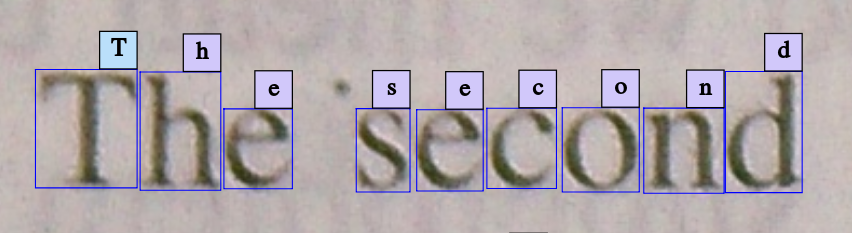
\includegraphics[height=4cm]{images/book-example-02.png}
    \caption{Primjer vizualizacije rezultata koji vraća OCR sustav.}
    \label{fig:book-example-02}
\end{figure}

\pagebreak


\begin{lstlisting}[caption={Primjer OCR rezultata u JSON formatu. Ulaz u sustav za određivanje strukture teksta.},label={lst:ocr-result-json-01}]
{
    "ocr_result": {
        "lines": [
            {
                "chars": [
                    {
                        "x": 25.95604,
                        "y": 17.30562,
                        "width": 10.64438,
                        "height": 16.60289,
                        "value": 48
                    },
                    {
                        "x": 19.77133,
                        "y": 1.28793,
                        "width": 16.07777,
                        "height": 10.76925,
                        "value": 77
                    },
                    {
                        "x": 5.50248,
                        "y": 2.84320,
                        "width": 12.13375,
                        "height": 15.60966,
                        "value": 73
                    },
                    {
                        "x": 3.19550,
                        "y": 19.67606,
                        "width": 14.94088,
                        "height": 20.78798,
                        "value": 91
                    },

                ]
            }
        ]
    }
}
\end{lstlisting}

\pagebreak

\section{Zahtjevi sustava}
Sustav za određivanje strukture teksta (u daljenjem tekstu: \emph{Sustav}) treba za dobiveni OCR rezultat u JSON formatu vratiti novi
rezultat u JSON formatu koji će znakove grupirati u linije i koji će unutar linija biti poredani
s lijeva na desno. Također, linije moraju biti sortirane tako da se najviša linija u dokumentu nalazi
na prvom mjestu.

Osim grupiranja linija, sustav treba odrediti gdje se nalazi razmak između riječi.
Od sustava se očekuje da između dva znaka, gdje smatra da završava prethodna i počinje nova
riječ, ubaci novi znak bjeline čija je vrijednost \engl{value} $32$ dok ostale informacije
mogu biti prozivoljne.

Isječak \ref{lst:ocr-result-json-02} prikazuje primjer izlaza iz sustava za dani ulaz
iz Isječka \ref{lst:ocr-result-json-01}. Sustav je znakove grupirao u dvije linije i
između prvog i zadnjeg znaka u drugoj liniji je ubacio znak bjeline. Vrijednost znaka
bjeline je zahtijevana vrijednost $32$. Ostale informacije znaka bjeline mogle su biti
proizvoljne, međutim, sustav im je dodijelio sljedeće smislenije vrijednost:

\begin{itemize}
    \item[$\bullet$] $x$ - horizontalna pozicija gornjeg desnog kuta lijevog znaka,
    \item[$\bullet$] $y$ - vertikalna pozicija gornjeg lijevog kuta desnog znaka,
    \item[$\bullet$] $width$ - horizontalna udaljenost između gornjeg desnog kuta lijevog
                               znaka i gornjeg lijevog kuta desnog znaka,
    \item[$\bullet$] $height$ - visina lijevog znaka.
\end{itemize}

Pod \emph{lijevi znak} podrazumijeva se na znak koji se nalazi prije znaka bjeline, a pod
\emph{desni znak} podrazumijeva se na znak koji se nalazi nakon znaka bjeline.

\

\begin{lstlisting}[caption={Primjer izlaza iz sustava za određivanje strukture teksta.},label={lst:ocr-result-json-02}]
{
    "ocr_result": {
        "lines": [
            {
                "chars": [
                    {
                        "x": 5.50248,
                        "y": 2.84320,
                        "width": 12.13375,
                        "height": 15.60966,
                        "value": 73
                    },
                    {
                        "x": 19.77133,
                        "y": 1.28793,
                        "width": 16.07777,
                        "height": 10.76925,
                        "value": 77
                    }
                ]
            },
            {
                "chars": [
                    {
                        "x": 3.19550,
                        "y": 19.67606,
                        "width": 14.94088,
                        "height": 20.78798,
                        "value": 91
                    },
                    {
                        "x": 18.13638,
                        "y": 19.67606,
                        "width": 7,81966,
                        "height": 20.78798,
                        "value": 32
                    }
                    {
                        "x": 25.95604,
                        "y": 17.30562,
                        "width": 10.64438,
                        "height": 16.60289,
                        "value": 48
                    }
                ]
            }
        ]
    }
}
\end{lstlisting}

\chapter{Skup podataka za testiranje}
\label{chap:skup-padataka-za-testiranje}

Skup podataka za testiranje (u daljnjem tekstu: \emph{podatci})
sustava sastoji se od slika, JSON datoteka i tekstualnih datoteka.
U sklopu ovog završnog rada razvijeni sustav za određivanje strukture teksta
rješavati će problem određivanja strukture teksta na računima iz trgovine i
sadržaja iz knjiga.

\section{Slike}
\label{sec:slike}

Podatci za testiranje sustava sadrže $100$ slika računa
(Slika \ref{fig:receipt-example-04}) i $34$ slike sadržaja iz knjiga (Slika \ref{fig:book-example-03}).

\

\begin{figure}[htb]
    \centering
    \captionsetup{justification=centering,margin=2cm}
    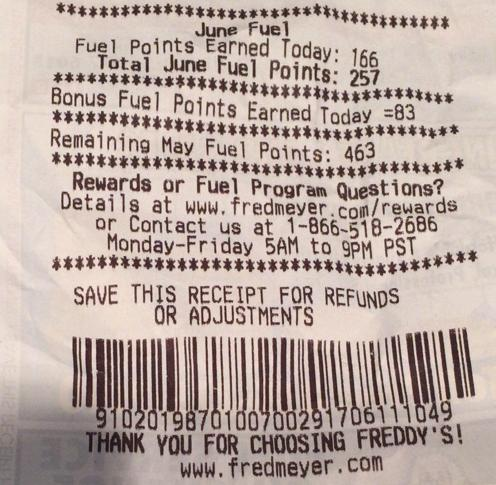
\includegraphics[height=8cm]{images/receipt-example-04.jpg}
    \caption{Primjer slike računa za koji će se rješavati problem određivanja strukture teksta.}
    \label{fig:receipt-example-04}
\end{figure}

\pagebreak

\begin{figure}[htb]
    \centering
    \captionsetup{justification=centering,margin=2cm}
    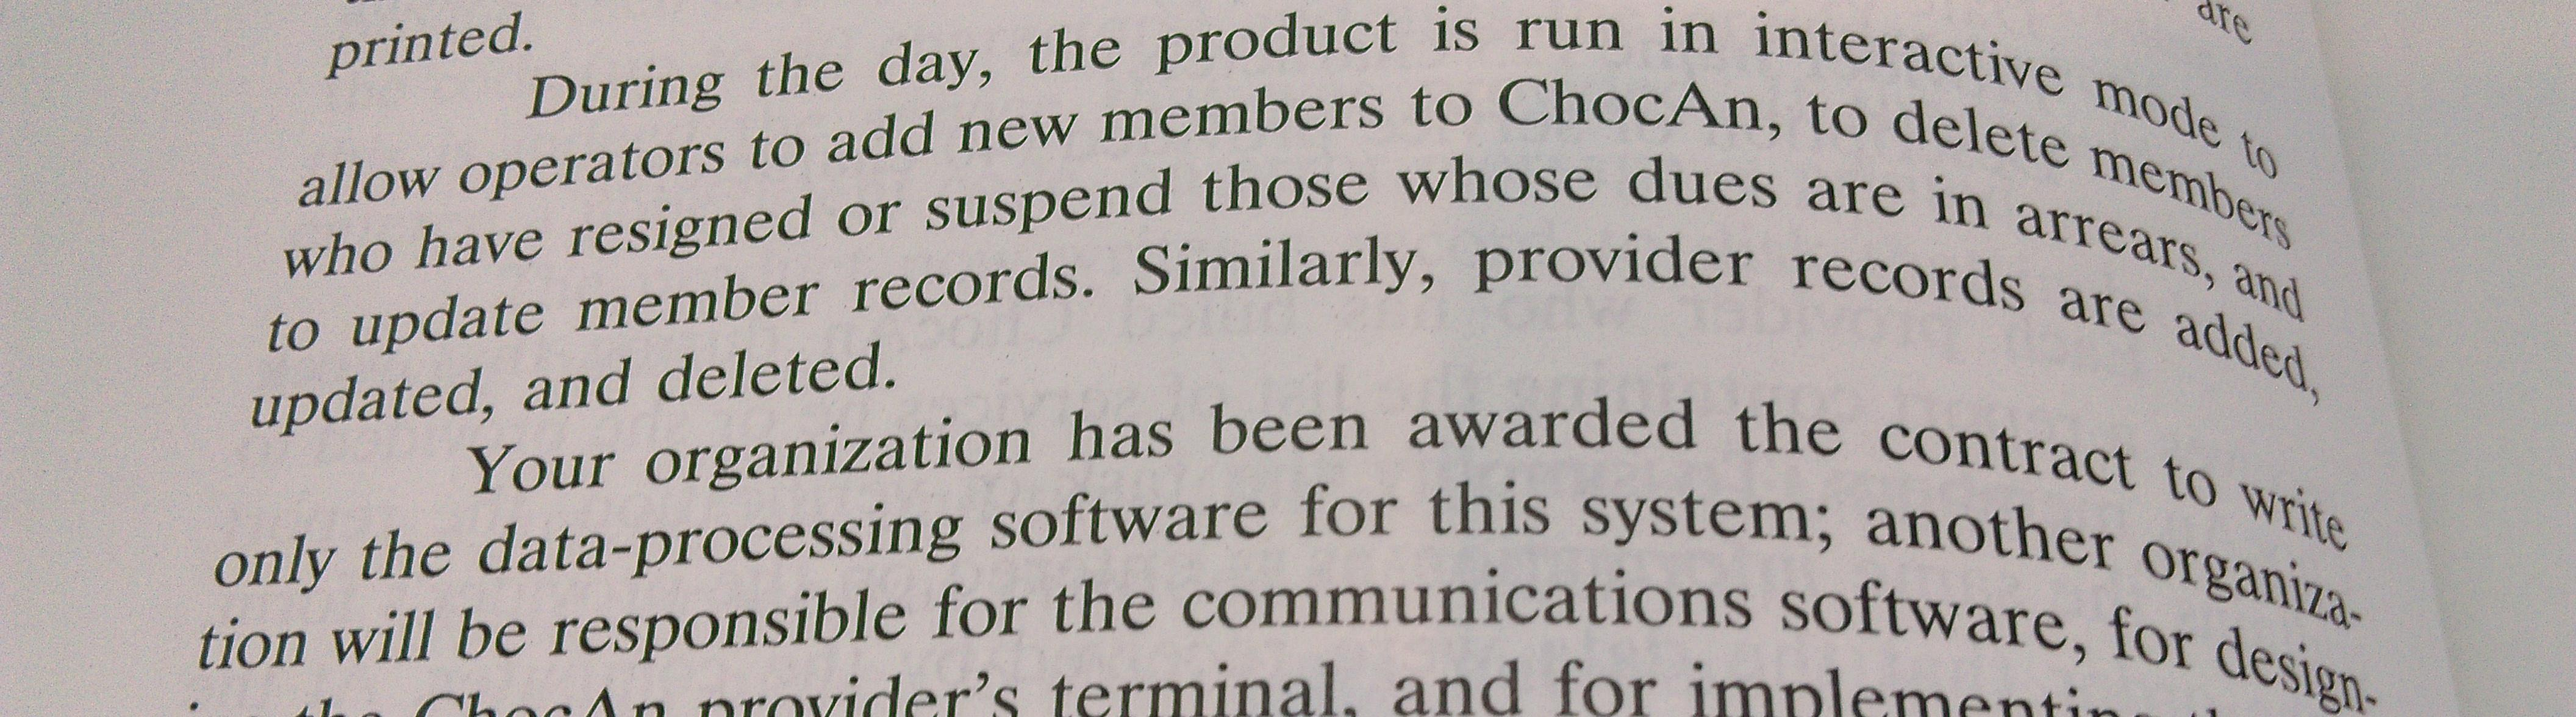
\includegraphics[width=\textwidth]{images/book-example-03.jpg}
    \caption{Primjer slike sadržaja iz knjige za koji će se rješavati problem određivanja strukture teksta.}
    \label{fig:book-example-03}
\end{figure}

Svaki znak na svakoj slici je \textbf{ručno} označen i klasificiran. Na slikama računa
označeno je ukupno $85068$ znakova, a na slikama sadržaja iz knjiga označeno je ukupno
$25092$ znaka. Ručno označeni podatci oponašaju rezultate OCR sustava koji predstavljaju ulaz u
sustav za određivanje strukture teksta.

Omeđujući pravokutnici označenih znakova predstavljaju područje koje označeni znak
zauzima na slici. Stranice omeđujućih pravokutnika su uvijek paralelne sa rubovima slike.
Slika \ref{fig:book-example-04} prikazuje isječak slike, sadržaja iz knjige, na kojoj
su znakovi ukošeni, a stranice njihovih omeđujućih znakova paralelne su sa rubovima slike.
Možemo uočiti kako je moguće da se dva susjedna omeđujuća pravokutnika preklapaju.

\

\begin{figure}[htb]
    \centering
    \captionsetup{justification=centering,margin=2cm}
    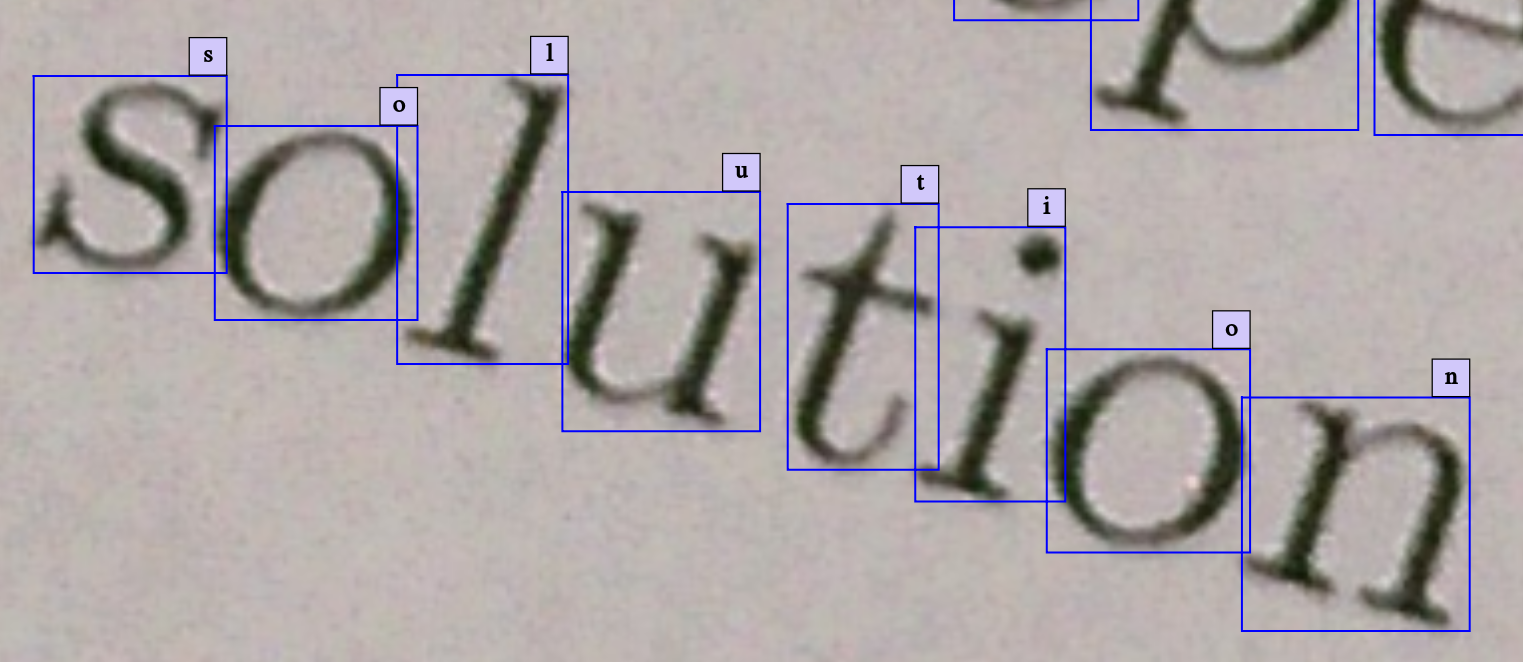
\includegraphics[width=\textwidth]{images/book-example-04.png}
    \caption{Primjer slike s kosim tekstom. Vizualizacija OCR rezultata. Omeđujući pravokutnici su uvijek paralelni s rubovima slike.}
    \label{fig:book-example-04}
\end{figure}

\section{JSON datoteke}
Slike opisane u \ref{sec:slike} \textbf{ne predstavljaju} ulaz u sustav za određivanje strukture
teksta. Nakon označavanja slika podatci o označavanju svake slike se izvoze i pohranjuju u JSON datoteke.
JSON datoteka u kojoj su zapisani podatci o označavanju Slike \ref{fig:receipt-example-04}
prikazana je u Isječku \ref{lst:ocr-result-json-03}. Početna tri ključa
\lstinline{meta}, \lstinline{tags} i \lstinline{crop} predstavljaju dodatne informacije
o označenoj slici i mogu se zanemariti. Zbog specifičnosti sustava za označavanje
slika i načina na koji on pohranjuje informacije o označavanju, svi označeni
znakovi će biti smješteni u jednu liniju u nasumičnom poretku, a ta linija
će biti smještena u jedan blok. Za svaki znak dostupna je informacija o Unicode
vrijednosti znaka koja je smještena pod ključem \lstinline{value}. Dodatno, za
svaki znak dostupna je informacija o poziciji i veličini njegovog omeđujućeg pravokutnika
\engl{bounding box}. Za svaki omeđujući pravokutnik poznate su sljedeće informacije:
\begin{itemize}
    \item[$\bullet$] $x$ - horizontalna pozicija gornjeg lijevog kuta,
    \item[$\bullet$] $y$ - vertikalna pozicija gornjeg lijevog kuta,
    \item[$\bullet$] $width$ - širina i
    \item[$\bullet$] $height$ - visina.
\end{itemize}

Kako vrijednost $x$ omeđujućeg pravokutnika raste tako je znak bliže desnom rubu slike.
Čim je vrijednost $y$ omeđujućeg pravokutnika veća time je znak niže na slici.
Sve informacije o omeđujućem pravokutniku su vrijednosti iz skupa nenegativnih realnih
brojeva.

Dodatne informacije dostupne za svaki znak smještene u ključeve
\lstinline{font} i \lstinline{quality} mogu se zanemariti.

\

\begin{lstlisting}[caption={JSON datoteka s podatcima o označavanju Slike \ref{fig:receipt-example-04}.},label={lst:ocr-result-json-03}]
{
    "meta": {
        "retailer": "Fred Meyer",
        "validation_type": "turk-multiple",
        "group": "ibotta-june-turk-multiple"
    },
    "tags": [
        "ibotta-june-turk-multiple"
    ],
    "crop": {
        "x": 90.0,
        "y": 209.0,
        "width": 496.0,
        "height": 485.0
    },
    "ocr_result": {
        "blocks": [
            {
                "lines": [
                    {
                        "chars": [
                            {
                                "value": 42,
                                "quality": 100,
                                "font": "unknown",
                                "bounding_box": {
                                    "x": 55.678818,
                                    "y": 1.7737274,
                                    "width": 10.0,
                                    "height": 12.452545
                                }
                            },
                            {
                                "value": 42,
                                "quality": 100,
                                "font": "unknown",
                                "bounding_box": {
                                    "x": 66.28284,
                                    "y": 3.0,
                                    "width": 10.434326,
                                    "height": 12.565659
                                }
                            },
                            // ostalih 585 znakova...
                        ]
                    }
                ]
            }
        ]
    }
}
\end{lstlisting}

\chapter{Algoritmi za određivanje strukture teksta}
U ovom poglavlju trebaš napisati na koji način je podijeljen sustav za određivanje
strukture teksta (\emph{aligner} i \emph{spacer}). Opisati način rada svakog
i njihovu suradnju. Opisati što se očekuje od \emph{alignera}, a što od \emph{spacera}.

\chapter{Rezultati i analiza}
\section{Metrike}
Opisati metrike koje su korištene za određivanje \emph{fitnesa} layoutera.
Zašto baš ta metrika, a ne neka druga. Objasniti prednosti i mane takve metrike
i koje su posljedice njezina korištenja.

\section{Brojke}
Brojke rezultata, grafovi ili tablice.

\section{Analiza}
Analiza rezultata. Zašto \emph{aligner} radi, a zašto ne. Isto tako i za
\emph{spacer}. Pokazati gdje \emph{aligner} griješi i analizirati zašto. Isto i za
\emph{spacer}.

\chapter{Daljnji rad}
Opisati što se može napraviti u bližoj budućnosti da rezultati budu bolji.
Definitvno spomenuti potrebu za izgradnjom boljeg skupa podataka i definiranja
metrike. Istaknuti prednosti takvog novog skupa podataka.

\chapter{Dodaci}
U dodacima rada opisati strukturu \emph{test-data} direktorija. Opisati
na koji način čitatelj može reproducirati rezultate i kako može isprobati rad
\emph{Layouter} na nekom svom skupu podataka. Pogledaj kako se ispravno dodaju
dodaci i u kojem dijelu rada dodatak mora biti.

\chapter{Zaključak}

\bibliography{literatura}
\bibliographystyle{fer}

\begin{sazetak}

\kljucnerijeci{}
\end{sazetak}

\engtitle{Text Layout Analysis System Based on Individual Character Positions}
\begin{abstract}

\keywords{}
\end{abstract}

\end{document}
